\documentclass[10pt]{beamer}

\usepackage[utf8]{inputenc}
\usepackage[italian]{babel}
% \usepackage[T1]{fontenc}

\usepackage{datetime2}
\DTMsetdatestyle{ddmmyyyy}
\DTMsetup{datesep=/}

\usepackage{minted}
\usemintedstyle{one-dark}

\usetheme[progressbar=frametitle]{metropolis}
\usepackage{appendixnumberbeamer}

\usepackage{booktabs}
\usepackage[scale=2]{ccicons}

\usepackage{graphicx}
\usepackage{subcaption}

\usepackage{pgfplots}
\usepgfplotslibrary{dateplot}

\usepackage{hyperref}

\usepackage{xspace}
\newcommand{\themename}{\textbf{\textsc{metropolis}}\xspace}

\title{Pydoku}
\subtitle{Un risolutore di sudoku in Python con OpenCV}
\date{\DTMDisplaydate{2022}{07}{22}{}}
\author{Simone Fidanza}
\institute{Università degli studi di Bari ``Aldo Moro''}

\begin{document}

\maketitle


\section[Introduzione]{Introduzione}
\begin{frame}[fragile]{Pydoku}
    Pydoku è un risolutore di sudoku che fa utilizzo di librerie come OpenCV,
    TensorFlow, Keras e NumPy. Il programma estrae le cifre dall'immagine di
    una griglia, la ricostruisce digitalmente e infine risolve il sudoku.
\end{frame}


\section{Modello}
\begin{frame}{Modello di Machine Learning}
    Il modello di Machine Learning che è stato utilizzato si ispira alla rete
    neurale LeNet\(5\), alla quale sono stati aggiunti vari layers fino ad
    arrivare ad un totale di \(10\).
%
    \begin{figure}[b]
        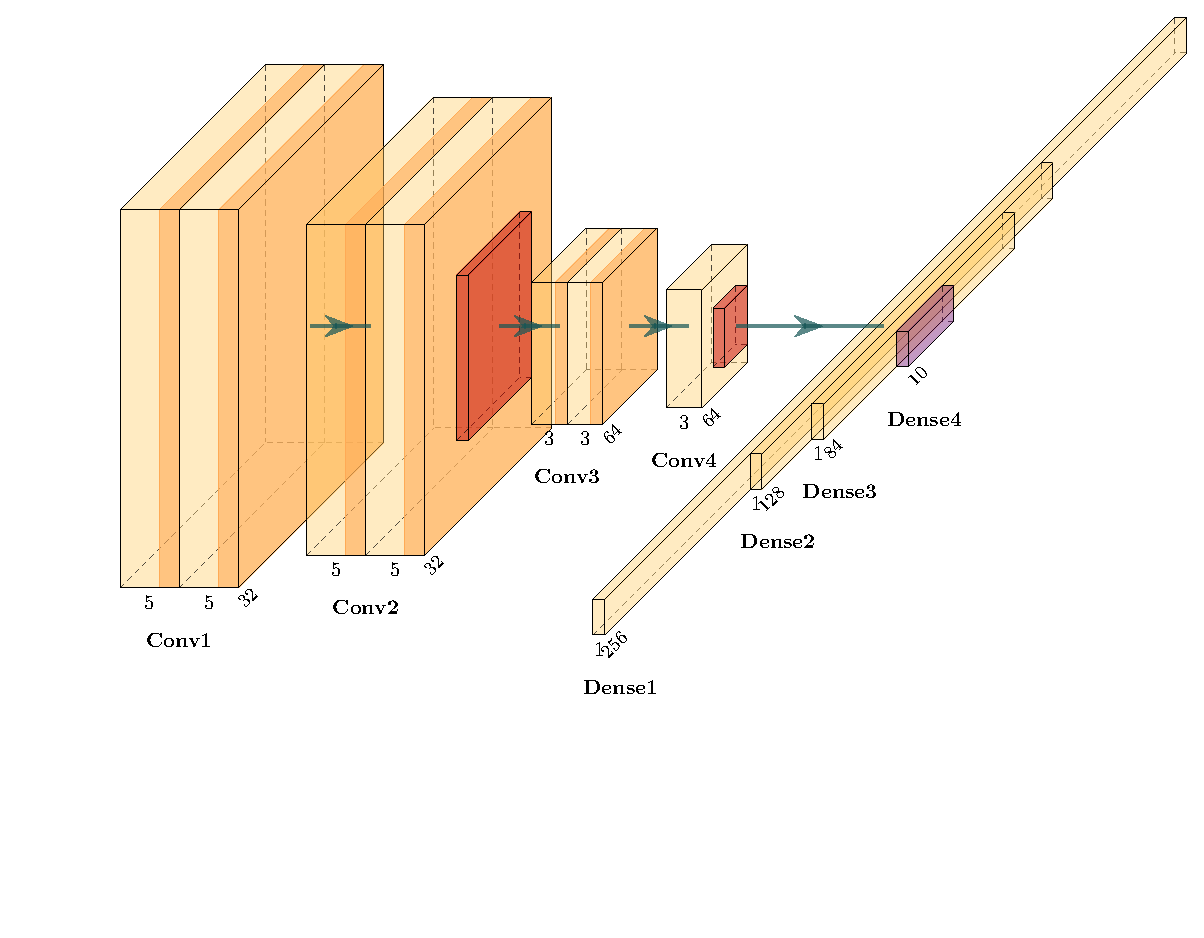
\includegraphics[width=0.6\textwidth, trim = 1cm 4.5cm 0cm 1cm]{architecture.pdf}
        \caption{Visualizzazione dell'architettura di LeNet\(5\)+}\label{fig:lenet}
    \end{figure}
\end{frame}


\section{Localizzazione della griglia}
\begin{frame}[fragile]{Pre-elaborazione dell'immagine}
    Per localizzazione la griglia del sudoku è necessario pre-elaborare
    l'immagine in modo tale che essa diventi un'immagine binaria.
%
    \begin{figure}
        \def\subwidth{0.50}
        \def\imgwidth{0.55}
        \centering
        \begin{subfigure}[b]{\subwidth\linewidth}
            \centering
            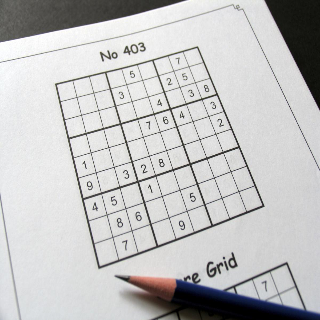
\includegraphics[width=\imgwidth\linewidth]{imgs/input.png}
            \caption{Originale}\label{subfig:input}
        \end{subfigure}%%
        \begin{subfigure}[b]{\subwidth\linewidth}
            \centering
            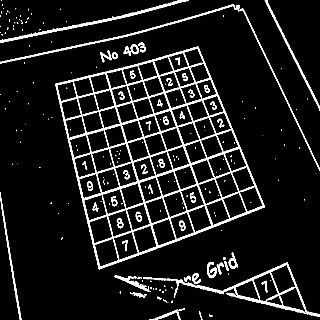
\includegraphics[width=\imgwidth\linewidth]{imgs/process_out.png}
            \caption{Pre-elaborazione}\label{subfig:preprocess}
        \end{subfigure}
        \caption{Processo di pre-elaborazione dell'immagine}\label{fig:pre_process}
    \end{figure}
\end{frame}


\begin{frame}[fragile]{Individuazione della griglia e deformazione dell'immagine}
    Per individuare la griglia è stata utilizzata la funzione
    \mintinline{py3}{cv2.findContours()}. È stato assunto che il più grande dei
    bordi fosse il bordo della griglia del sudoku. Approssimando questo
    poligono con \mintinline{py3}{cv2.approxPolyDP()} sono stati ottenuti gli
    angoli della griglia. Usando sia quest'ultimi che
    \mintinline{py3}{cv2.getPerspectiveTransform()} che
    \mintinline{py3}{cv2.WarpPerspective()} l'immagine viene deformata e resa
    piana.
%
    \begin{figure}
        \def\subwidth{0.50}
        \def\imgwidth{0.50}
        \centering
        \begin{subfigure}[b]{\subwidth\linewidth}
            \centering
            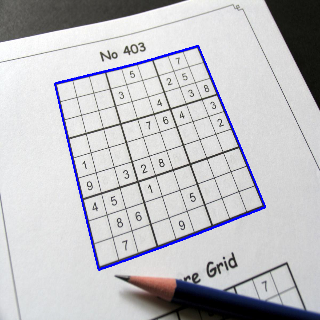
\includegraphics[width=\imgwidth\linewidth]{imgs/grid.png}
            \caption{Individuazione della griglia}\label{subfig:grid}
        \end{subfigure}%%
        \begin{subfigure}[b]{\subwidth\linewidth}
            \centering
            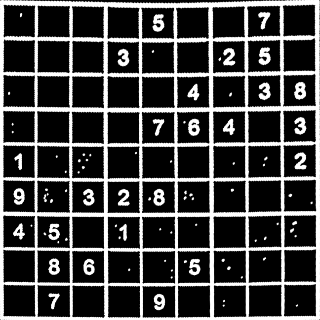
\includegraphics[width=\imgwidth\linewidth]{imgs/warp.png}
            \caption{Deformazione e appiattimento}\label{subfig:warp}
        \end{subfigure}
        \caption{Processo di deformazione dell'immagine}\label{fig:warp_process}
    \end{figure}
\end{frame}


\section{Analisi delle celle}
\begin{frame}[fragile]{Estrazione delle cifre}
    Per estrarre le cifre, la griglia piana viene divisa in \(81\) immagini.
    Tramite un algoritmo vengono scartate le immagini che non contengono alcun
    numero. Le immagini che invece ne contengono uno, vengono analizzate dalla
    rete neurale che effettua una predizione.
    Se la cifra non è presente, viene inserito \mintinline{py3}{0} nella lista,
    altrimenti viene inserita la predizione.
%
    \begin{figure}
        \def\subwidth{0.50}
        \def\imgwidth{0.50}
        \centering
        \begin{subfigure}[b]{\subwidth\linewidth}
            \centering
            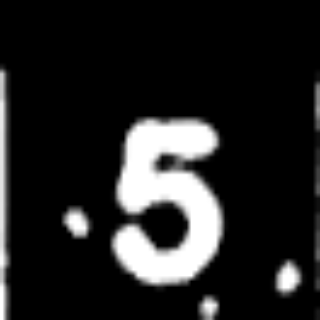
\includegraphics[width=\imgwidth\linewidth]{imgs/cell_pre.png}
            \caption{Prima}\label{subfig:cell_pre}
        \end{subfigure}%%
        \begin{subfigure}[b]{\subwidth\linewidth}
            \centering
            
\includegraphics[width=\imgwidth\linewidth]{imgs/cell_post.png}
            \caption{Dopo}\label{subfig:cell_post}
        \end{subfigure}
        \caption{Processo di estrazione delle cifre}\label{fig:extraction}
    \end{figure}
\end{frame}


\section{Risoluzione del sudoku}

\begin{frame}[fragile]{Soluzione}
    Dopo aver ricostruito ``artificialmente'' la griglia del sudoku, questa
    viene passata all'algoritmo di risoluzione del sudoku.
    Successivamente la griglia viene mostrata a schermo.
\end{frame}

\section{Limitazioni note}

\begin{frame}[fragile]{Limitazioni}
    \begin{itemize}
        \item nel deformare e appiattire un'immagine già piana, questa viene
            ruotata di \(90^\circ\) in senso orario;
        \item nel determinare se una cella è priva o meno di numero, poiché
            l'algoritmo si basa sul numero di pixel bianchi, a volte
            questo può considerare vuote celle che contengono dei numeri;
        \item nel predirre le cifre, la rete neurale a volte confonde il numero
            \(1\) col numero \(7\) e raramente il numero \(6\) col numero \(5\)
            o \(8\).
    \end{itemize}
\end{frame}

\begin{frame}{Riepilogo}
    Il codice sorgente del progetto è disponibile su

    \begin{center}
        \href{https://www.github.com/sRavioli/pydoku}{github.com/sRavioli/pydoku}
    \end{center}

    Il progetto è sotto licenza \href{https://www.gnu.org/licenses/gpl-3.0.html}{GNU General Public License v3.0}.
\end{frame}

\end{document}
